
Antud töö eesmärgiks oli luua masinnägemise rakendus selliselt, et ta oleks võimeline võimalikult varieeruvatel juhtkontrolleritel jooksma. Selleks oli tarvis pakendada rakendus ära nii, et kontrolleris olemasolevaid seadistusi ei muudetaks ega lisanduvaid tarkvarasid ei installitaks. Samal ajal pidi rakendus olema võimeline vastavalt riistvarale valima sisemised seadistused nii, et tarkvara töö oleks võimalikult riistvaralähedane ehk optimeeritud, tagades seetõttu oma universaalsuse. Rakenduse sisendid pidid olema kasutajale lihtsasti interpreteeritavad ning hästi dokumenteeritud, vältimaks valesid sisendeid. Tarkvara takerdunud töö korral oli tähtsal kohal korrektse ja informatiivse veateate kuvamine. Lihtsustatud versioon seadme tarkvaralisest lahendusest on töö autori poolt avaldatud, saadaval ning pidevalt uuendamisel Githubis \cite{ref56}.

\section{Töökeskkond}\label{tuxf6uxf6keskkond}

Tarkvara arendamine ning masinnägemise protsesside töö toimub isoleeritud keskkonnas, mis võimaldab testida tarkvara erinevate riistvara konfiguratsioonidega süsteemidel. Samuti tagab selline arendusvõte turvalisuse ja stabiilsuse poolelt hostsüsteemi tarkvara ning oleku puutumatuse. Konteinerdamine võimaldab ühel seadmel jooksutada mitut rakendust, mis kõik võivad olla erinevate konfiguratsioonidega ning tarkvaradega, seejuures kasutaja poolt määratud otsese ligipääsuga hosti riistvarale (vt Joonis 5.1.1).

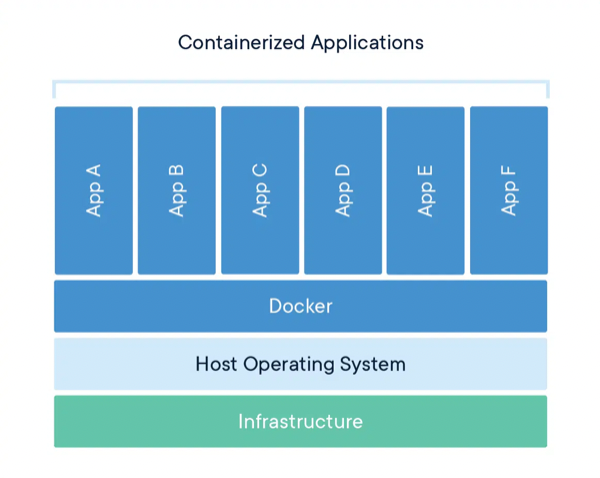
\includegraphics[width=4.67812in,height=3.72586in]{media/image13.png}

Joonis 5.1.1. Konteinerdatud rakenduste toimimise lihtsustatud skeem \cite{ref57}

Süsteemi arenduseks ja testimiseks loodi keskkond eraldiseisva arendusmasina peal, kasutades virtualiseerimiskeskkonda Dockerit \cite{ref58}. Aluseks võeti Nvidia NGC keskkonnast PyTorchi konteiner, mõeldud x86\_64 arhitektuuriga seadmetele \cite{ref59}. Selle sisse ehitati Jetsoni tarkvaraliste spetsiifilisustega analoogne keskkond ning loodi ka koodis arhitektuuripõhised funktsioonid, mis rakendusid vastavalt eripäradele arendussüsteemile ja toodangsüsteemile (vt Joonis 5.1.2 ja 5.1.3).

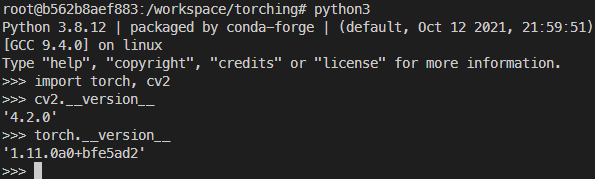
\includegraphics[width=6.10174in,height=1.83333in]{media/image14.png}

Joonis 5.1.2. Arendusmasina konteinerisse installeeritud tarkvarade versioonid, mis ühilduvad toodangmasina konteineri seisundiga kõige paremini

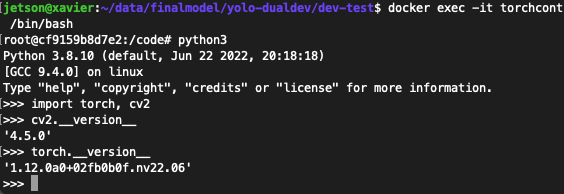
\includegraphics[width=6.09626in,height=2.09526in]{media/image15.png}

Joonis 5.1.3. Toodangsüsteemi konteineri tarkvarade versioonid

Toodangsüsteemi jaoks loodi samuti konteiner, mille põhjaks konfigureeriti samuti NGC keskkonnast konteiner, mis on üles ehitatud L4T (\emph{Linux for Tegra}) süsteemiga, spetsiifiliselt loodud aarch64 arhitektuuriga Jetson seadmetele \cite{ref60}. See konfigureeriti vastavalt masinnägemiseks vajalike lisateekide ning seoti riistvaral oleva närvivõrkude mudelite optimeerimise rakendusega TensorRT \cite{ref61}.

\section{Põhiprogramm}\label{puxf5hiprogramm}

Peamine töö toimub inferentsi skriptis (vt lihtsustatud Joonis 5.2.1, tehniline Joonis 5.2.3), millele kasutaja annab sisendiks närvivõrgumudeli ning selle vajalikud parameetrid, sisendstriimi (videofail või kaamera) ning vajadusel ka soovitud režiimi (videosalvestus või videoväljastuseta debugimiseks ja kiiruse kontrolliks mõeldud režiim) (vt Joonis 5.2.2)

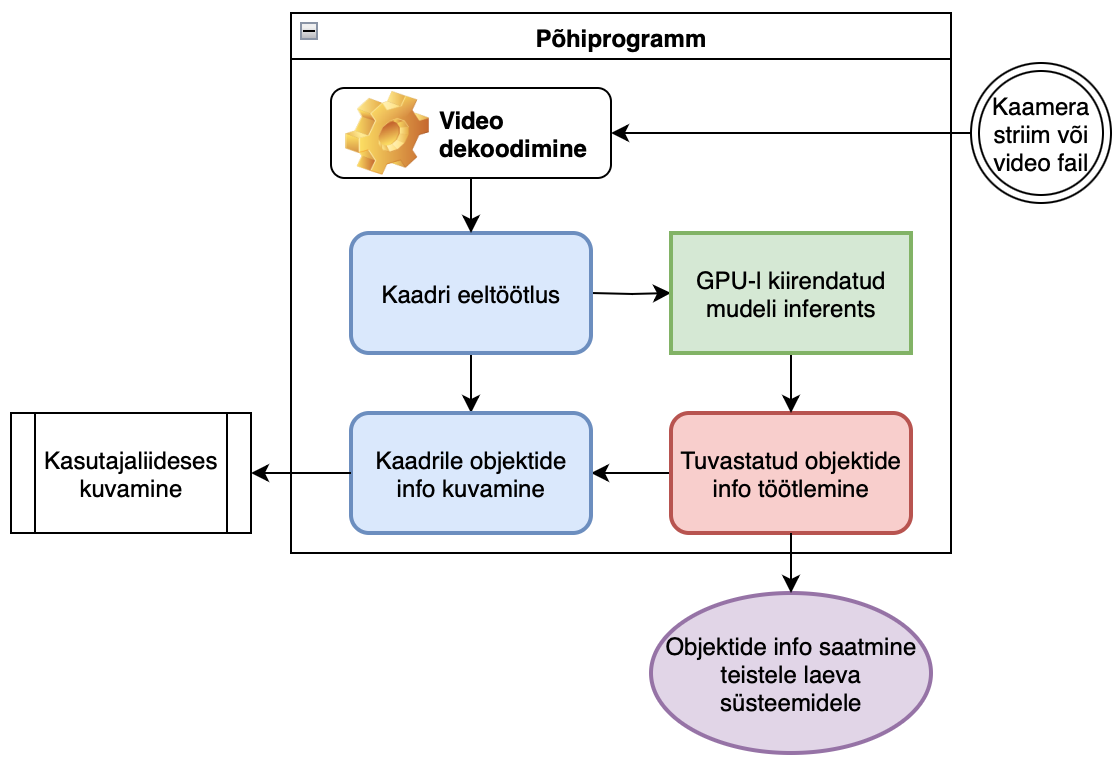
\includegraphics[width=6.00897in,height=4.07576in]{media/image16.png}

Joonis 5.2.1. Põhiprogrammi lihtsustatud plokkskeem

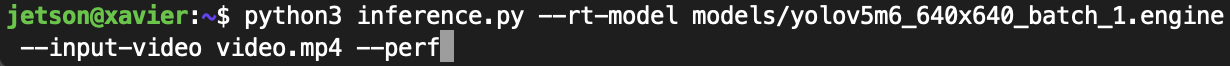
\includegraphics[width=6.10174in,height=0.33333in]{media/image17.png}

Joonis 5.2.2. Põhiprogrammi käitamise näide käsurealt

Pythoniga käitatakse skript nimega inference.py, millele antakse sisendiks TensorRT-ga optimeeritud mudel, nimega yolov5m6, sisendstriimiks antakse videofail video.mp4, samuti lülitatakse sisse performance režiim, mis käitab protsessi ilma veebiliidese videoväljundita kasutajale, selle abil on võimalik hinnata süsteemi latentsust ning otsest mõju Xavieri ressursside kasutusele.

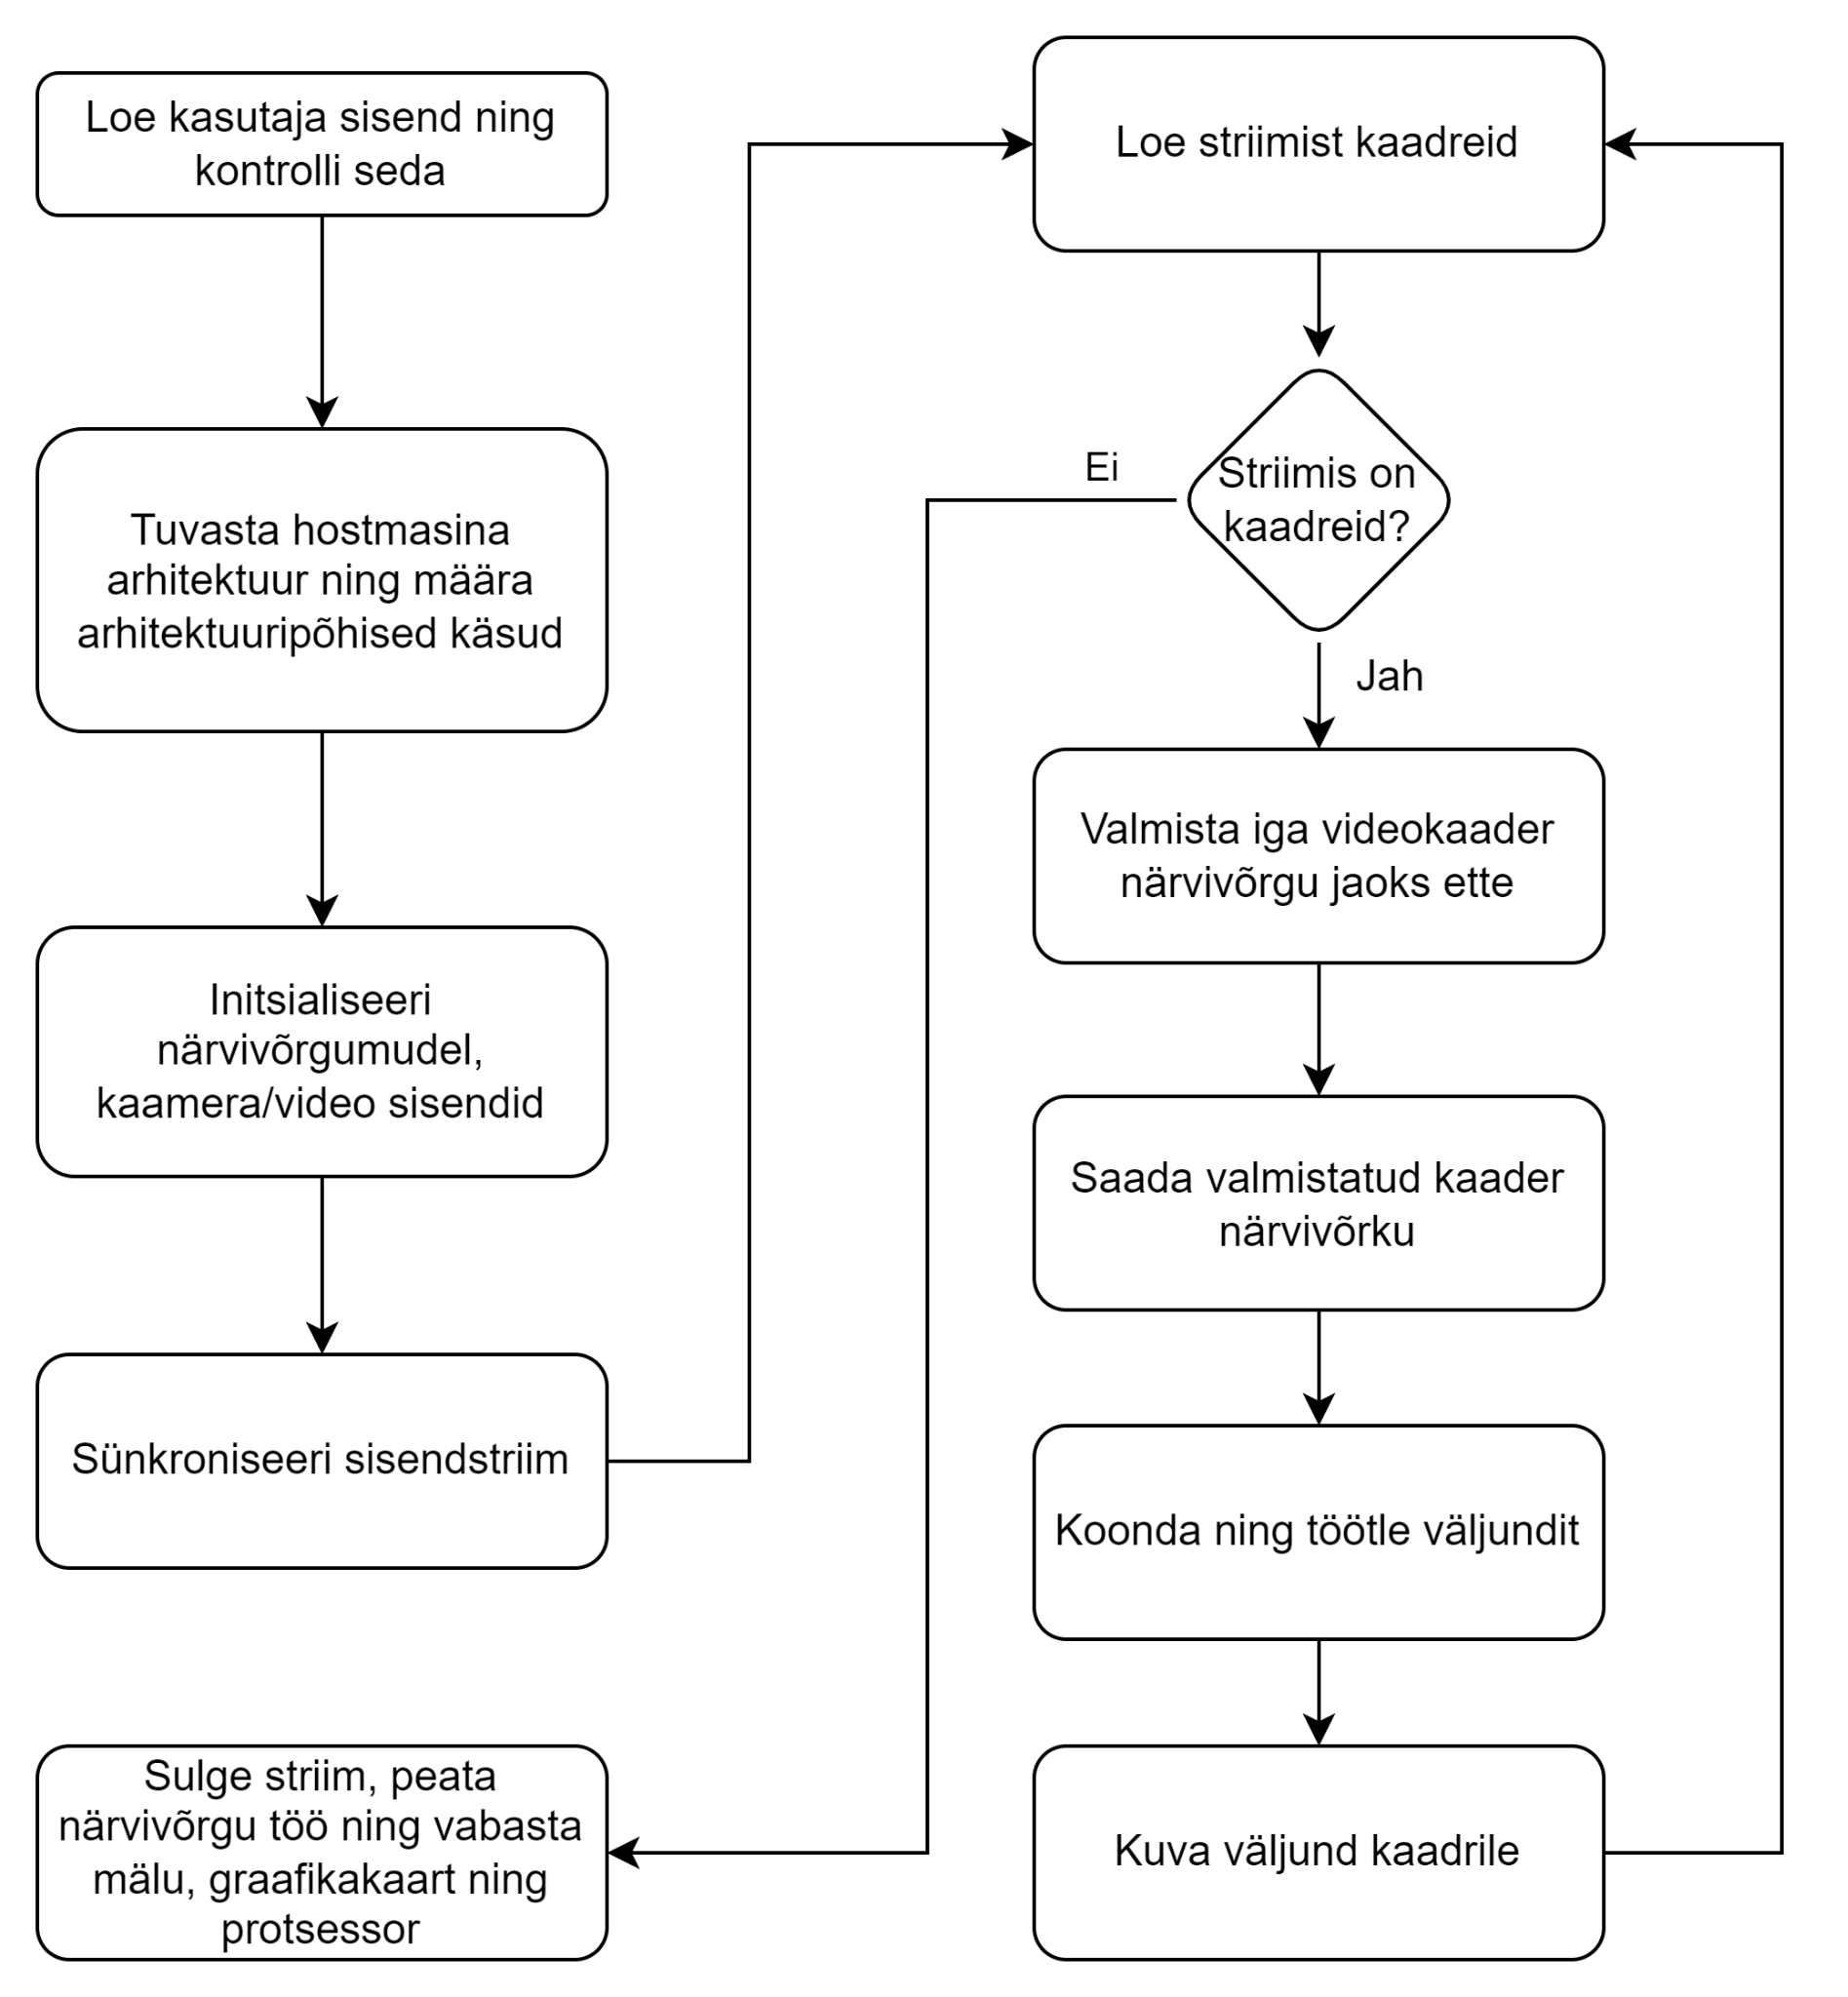
\includegraphics[width=5.71979in,height=6.17581in]{media/image18.png}

Joonis 5.2.3. Masinnägemise programmi toimimise lihtsustatud plokkskeem

Masina arhitektuuri tuvastamiseks kasutatakse pythoni moodulit, vastavalt millele rakendatakse vajalikud seadesätted skripti käitanud keskkonna jaoks. Arenduskeskkonnaks kasutatakse lauarvutit, mis on x86\_64 arhitektuuriga, mille seadistamisel initsialiseeritakse vastav videodekooder ning enkooder, samuti määratakse ka erikasutusel olev port ning kaameratest tuleva info jaoks skaleerimise parameeter (vt Joonis 5.2.4).

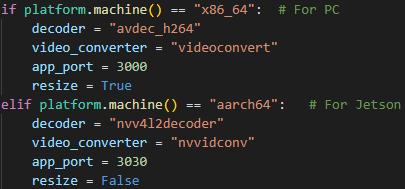
\includegraphics[width=4.21875in,height=1.96875in]{media/image19.png}

Joonis 5.2.4. Arhitektuuripõhiste parameetrite initsialiseerimine

Närvivõrgu mudel loetakse sisse kasutaja poolt defineeritud ``model'' parameetriga, mis kontrollib mudeli olemasolu ning faili formaati, antud juhul on mudeli formaadiks .engine tüüpi TensorRTga \cite{ref60} optimeeritud mudelid. Pärast mudeli formaadi kontrolli loetakse sisse mudeli parameetrite metadata, vastavalt millele allokeeritakse graafikakaardi mälu ning tuumade ressurss.

Kaameratest info lugemiseks kasutatakse Nvidia graafikakaardil asetsevat riistvarakiirendit Nvidia Video Decoder (NVDEC) \cite{ref62}, mis võimaldab protsessoril ja graafikakaardil tegeleda täielikult närvivõrgu haldamise ning andmete töötlusega.

Kaameratest saadud kaadrid skaleeritakse närvivõrgule sobivasse sisendformaati, seejärel toimub mudelis kaadritelt informatsiooni hankimine ning statistiliste väljundite formuleerimine. Seejärel saadetakse väljundinfo järeltöötlusesse, kus toimub tulemuste vormistamine ning kaadrile tuvastatud objektide asukohtade ning kindluse tõenäosuse kuvamine (vt Joonis 5.2.5). Seejärel loetakse sisse uus kaader ning programmi töö kordub kuni enam kaadreid sisse ei tule ehk kas kaamera töö lõpeb või kasutaja lõpetab programmi töö.

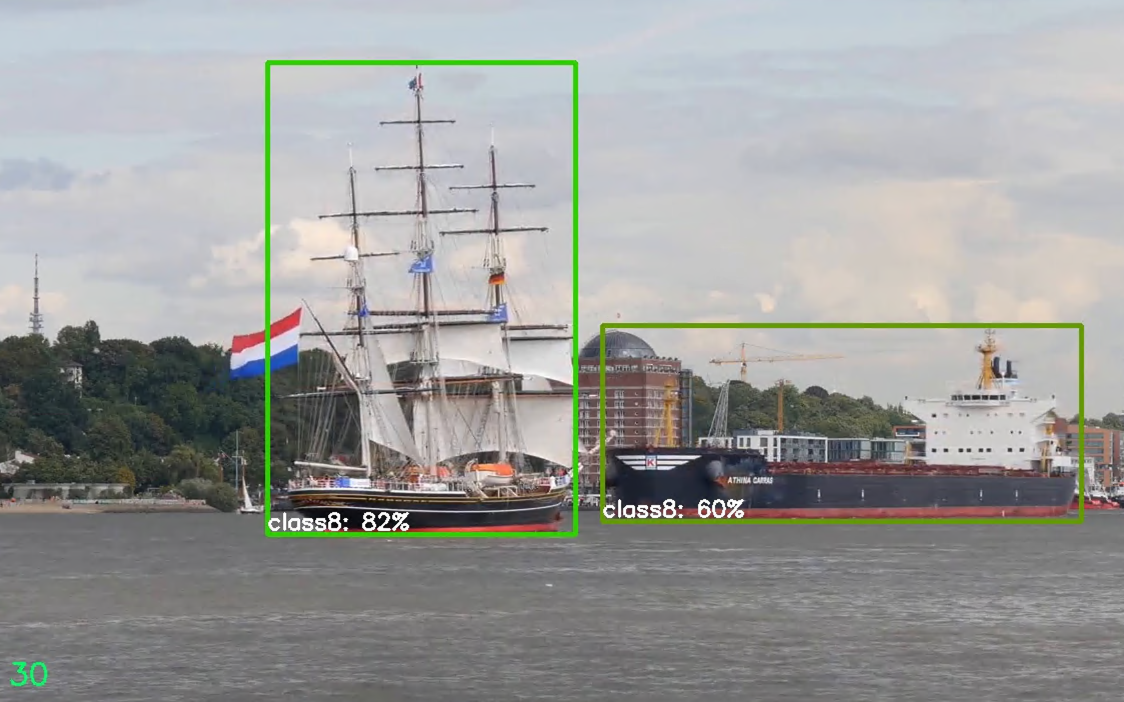
\includegraphics[width=5.98021in,height=3.72487in]{media/image20.png}

Joonis 5.2.5. Kaadrile kuvatud närvivõrgu poolt genereeritud ja töödeldud tuvastused (kastid ja nende sees olevad tuvastatud klassid koos tõenäosustega)

\section{Masinnägemise mudeli ja tarkvara optimeerimine}\label{masinnuxe4gemise-mudeli-ja-tarkvara-optimeerimine}

Masinnägemise rakenduse algfaasis esinesid mitmed probleemid nii kaameratelt sisendite lugemisel kui ka masinnägemise mudeli jooksutamisel riistvara peal.

Rakenduse esimeseks probleemiks oli kaameratelt tuleva striimi lugemine mitme sisendi korral, mis oli protsessorile koormav (kaadrite läbilaskevõime oli madal) ning seetõttu ka juhtkontrolleri temperatuur oli kõrge. Selle tagajärjena ei jätkunud ressurssi teistele seadmetele mis Jetsoniga suhtlesid (radari toimimine oli halvatud). Samuti ei olnud ka masinnägemine töövõimeline kuna kogu protsessor oli hõivatud kaameratelt tulevate kaadrite lugemise ning nende ümberskaleerimisega.

Selle lahendamiseks võeti kasutusele Jetsonisse integreeritud riistvaraline videodekooder NVDEC \cite{ref41}, OpenCV abil, millele anti ette kiirendusega gstreameri käsk, mis sisaldas endas sisendit ja videodekoodri kutsungit.

Teise probleemina ei olnud võimalik suuremaid masinnägemise mudeleid edukalt jooksutada, kuna mudelid laeti protsessori mällu ning marginaalne osa arvutuslikust tööst koos kaadrite töötlusega närvivõrgus kandus graafikakaardile (vt Joonis 5.3.1).

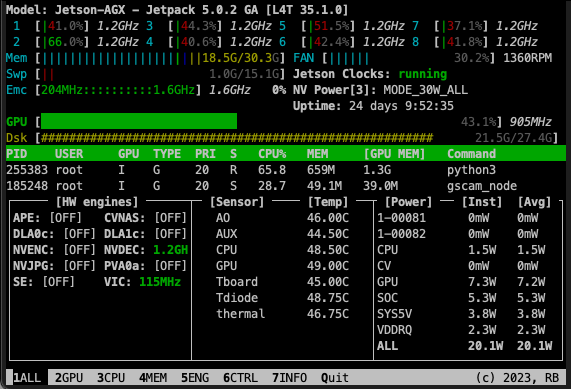
\includegraphics[width=5.94792in,height=4.05208in]{media/image21.png}Joonis 5.3.1. YOLOv5l, ühe sisendiga, resolutsioonil 640x640 pikslit, optimeerimata mudeli jooksmine ei utiliseeri kogu graafikakaarti, monitooringurakenduses jtop \cite{ref43}

Antud probleemile leiti lahenduseks Nvidia TensorRT tööriist, mis on võimeline sisendiks võtma mitmes formaadis närvivõrke ning need vastavalt olemasolevale riistvarale kiirendama. Antud tööriista kasutamisel valmistati närvivõrgud ette ONNX \cite{ref63} formaadis, mis on kõige universaalsem ning hõlpsasti kasutatav masinõppe mudelite interpreteerimise viis.

TensorRT tööpõhimõte on mudelis kvantiseerimine ehk mudeli parameetrite arvutusliku täpsuse vähendamine (nt 32lt ujukomaarvult, 16le ujukomaarvule), see võimaldab kasutada suure jõudlusega vektorarvutusi selleks spetsialiseeritud riistvaral marginaalsete mõjutustega mudeli täpsusele. Teisena toimub mudeli kärpimine ehk ebavajalike ning minimaalselt mudeli inferentsi tulemusi mõjutavate parameetrite eemaldamine, tehes mudeli mahtu väiksemaks, mille tõttu ka mudeli kiirus paraneb (vt peatükk 5.2).

Optimeerimiste tulemusena (vt Joonis 5.3.2) on:

\begin{itemize}
\item
  graafikakaardi kasutus tõusnud (43,1 \% langes 99,8 \%)
\item
  keskmine energiakasutus vähenenud 26,8 \% (20,1 W langes 14,7 W)
\item
  töötemperatuurid langenud 3,3 \% (46 ° langes 44,5 °)
\item
  mälu kasutus langenud 1,6 \% (18,5 GB langes 18,2 GB)
\end{itemize}

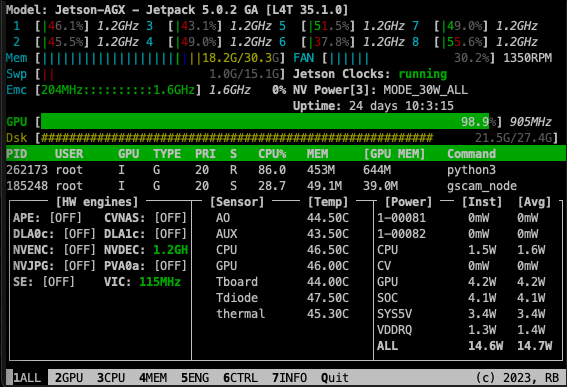
\includegraphics[width=5.90625in,height=4.03125in]{media/image22.png}Joonis 5.3.2. YOLOv5l, ühe sisendiga, resolutsioonil 640x640 pikslit, optimeeritud mudeli jooksmine utiliseerib kogu graafikakaardi
